\def\tightlist{}
\documentclass[dutch, biblatex]{deltares_report}
$if(highlighting-macros)$
$highlighting-macros$
$endif$
$if(csl-refs)$
% Pandoc citation processing
\newlength{\cslhangindent}
\setlength{\cslhangindent}{1.5em}
\newlength{\csllabelwidth}
\setlength{\csllabelwidth}{3em}
\newlength{\cslentryspacingunit} % times entry-spacing
\setlength{\cslentryspacingunit}{\parskip}
% for Pandoc 2.8 to 2.10.1
\newenvironment{cslreferences}%
  {$if(csl-hanging-indent)$\setlength{\parindent}{0pt}%
  \everypar{\setlength{\hangindent}{\cslhangindent}}\ignorespaces$endif$}%
  {\par}
% For Pandoc 2.11+
\newenvironment{CSLReferences}[2] % #1 hanging-ident, #2 entry spacing
 {% don't indent paragraphs
  \setlength{\parindent}{0pt}
  % turn on hanging indent if param 1 is 1
  \ifodd #1
  \let\oldpar\par
  \def\par{\hangindent=\cslhangindent\oldpar}
  \fi
  % set entry spacing
  \setlength{\parskip}{#2\cslentryspacingunit}
 }%
 {}
\usepackage{calc}
\newcommand{\CSLBlock}[1]{#1\hfill\break}
\newcommand{\CSLLeftMargin}[1]{\parbox[t]{\csllabelwidth}{#1}}
\newcommand{\CSLRightInline}[1]{\parbox[t]{\linewidth - \csllabelwidth}{#1}\break}
\newcommand{\CSLIndent}[1]{\hspace{\cslhangindent}#1}
\renewcommand{\FrontCover}{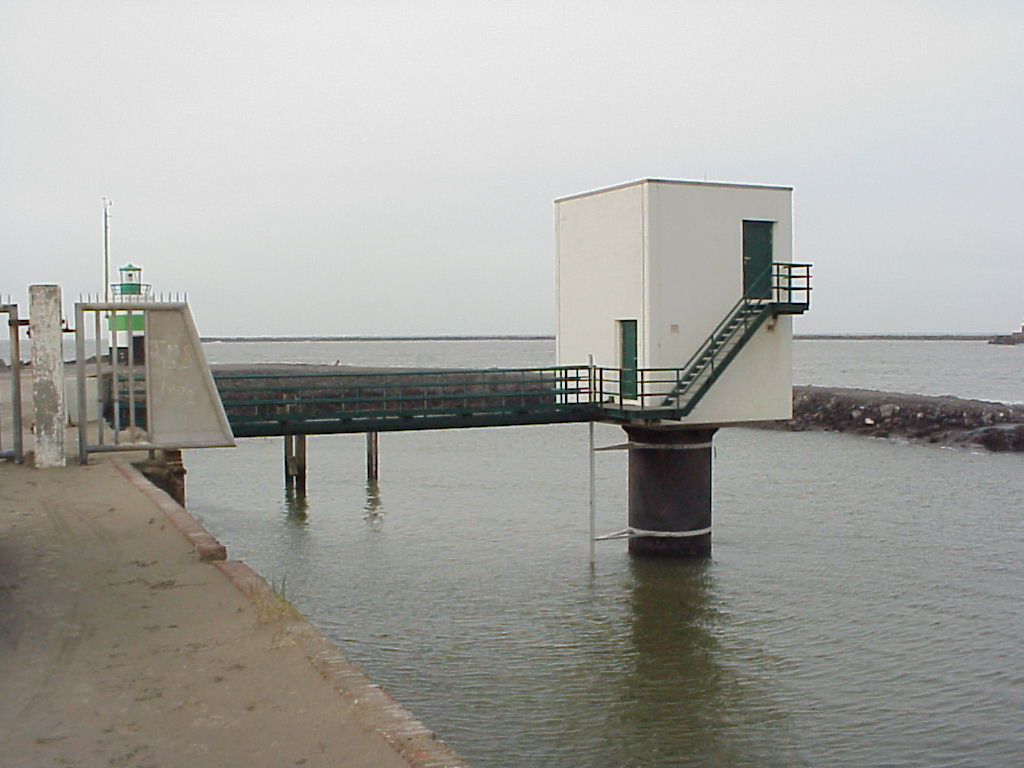
\includegraphics[width=182mm,height=182mm]
{figures/IJMDBTHVN.jpg}}
\coverPhoto{Meetstation IJmuiden, foto van nap-info. }
$endif$
\begin{document}
\title{Zeespiegelmonitor}
\subtitle{2022}
\author{Willem Stolte, Fedor Baart, Sanne Muis, Marc Hijma, Marcel Taal (Deltares)
Dewi Le Bars, Sybren Drijfhout (KNMI) met bijdragen van HKV.}
\partner{}

\client{Ministerie van Infrastructuur en Waterstaat/DG Water en Bodem}
\contact{}
\reference{}
\keywords{Zeespiegel, Zeespiegelstijging, Bodemdaling}

\version{1.0}
\date{27-03-2023}
\projectnumber{11208038}
\documentid{11209266-000-ZKS-0001}
\status{definitief}
\disclaimer{}
%\references{}

\authori{Willem Stolte, Fedor Baart, Sanne Muis, Marc Hijma, Marcel Taal (Deltares), Dewi Le Bars, Sybren Drijfhout (KNMI)}
\datei{03-27-2023}
\organisationi{Deltares}
\versioni{1.0}
\revieweri{Bart van den Hurk}
\approvali{Toon Segeren}
\publisheri{Deltares}

\summary{
Sinds 2014 onderhoudt Deltares in opdracht van Ministerie van I\&W de Zeespiegelmonitor. Doel is de stand en ontwikkeling van de zeespiegel vast te stellen, ter ondersteuning van het waterveiligheidsbeleid. Het gaat met name om de gemiddelde hoeveelheid jaarlijks te suppleren zand en het toetsen en ontwerpen van de primaire waterkeringen.

De Zeespiegelmonitor stelt jaarlijks de stand van de zeespiegel vast van de zes Nederlandse hoofdgetijdenstations (Delfzijl, Harlingen, Den Helder, IJmuiden, Hoek van Holland en Vlissingen), die continu de waterstand vastleggen/meten. De methodiek voor de Zeespiegelmonitor is in 2014 vastgesteld en berekent de langjarige trend. Bij deze berekening wordt rekening gehouden met de verschillende factoren die de fluctuaties in waterstanden beïnvloeden. Wind en getij zijn daarvan de belangrijkste. Het resultaat van de zeespiegelmonitor wordt representatief geacht voor de gemiddelde zeespiegelstijging in de komende ca 15 jaar. Iedere vier jaar wordt gerapporteerd over de waarnemingen en de onderzoeksresultaten. Dit is de derde rapportage.

In de vorige twee rapportages is geconcludeerd dat, cf.~de methodiek, een constante trend, sinds 1900, de beste beschrijving geeft van de trend. In deze rapportage wordt een andere conclusie onderbouwd/getrokken. De stijging van de zeespiegel langs de Nederlandse kust kan nu het best beschreven worden door een trend tot circa 1990 van 1.8 ± 0.1 mm/jaar, met een toename van de gemiddelde jaarlijkse stijging over de laatste 30 jaar van 2.9 ± 0.4 mm/jaar. Deze toename past bij de verwachting, op basis van de kennis over de wereldwijde stand van de zeespiegel, van een langzaam opbouwende versnelling van de zeespiegelstijging.

Voor de komende ca 15 jaar is een trend van 2.9 mm/jaar een verantwoorde benadering. De methodiek toegepast in de zeespiegelmonitor, is niet geschikt voor een berekening van de trend over de periode daarna.

\begin{figure}[h]

{\centering 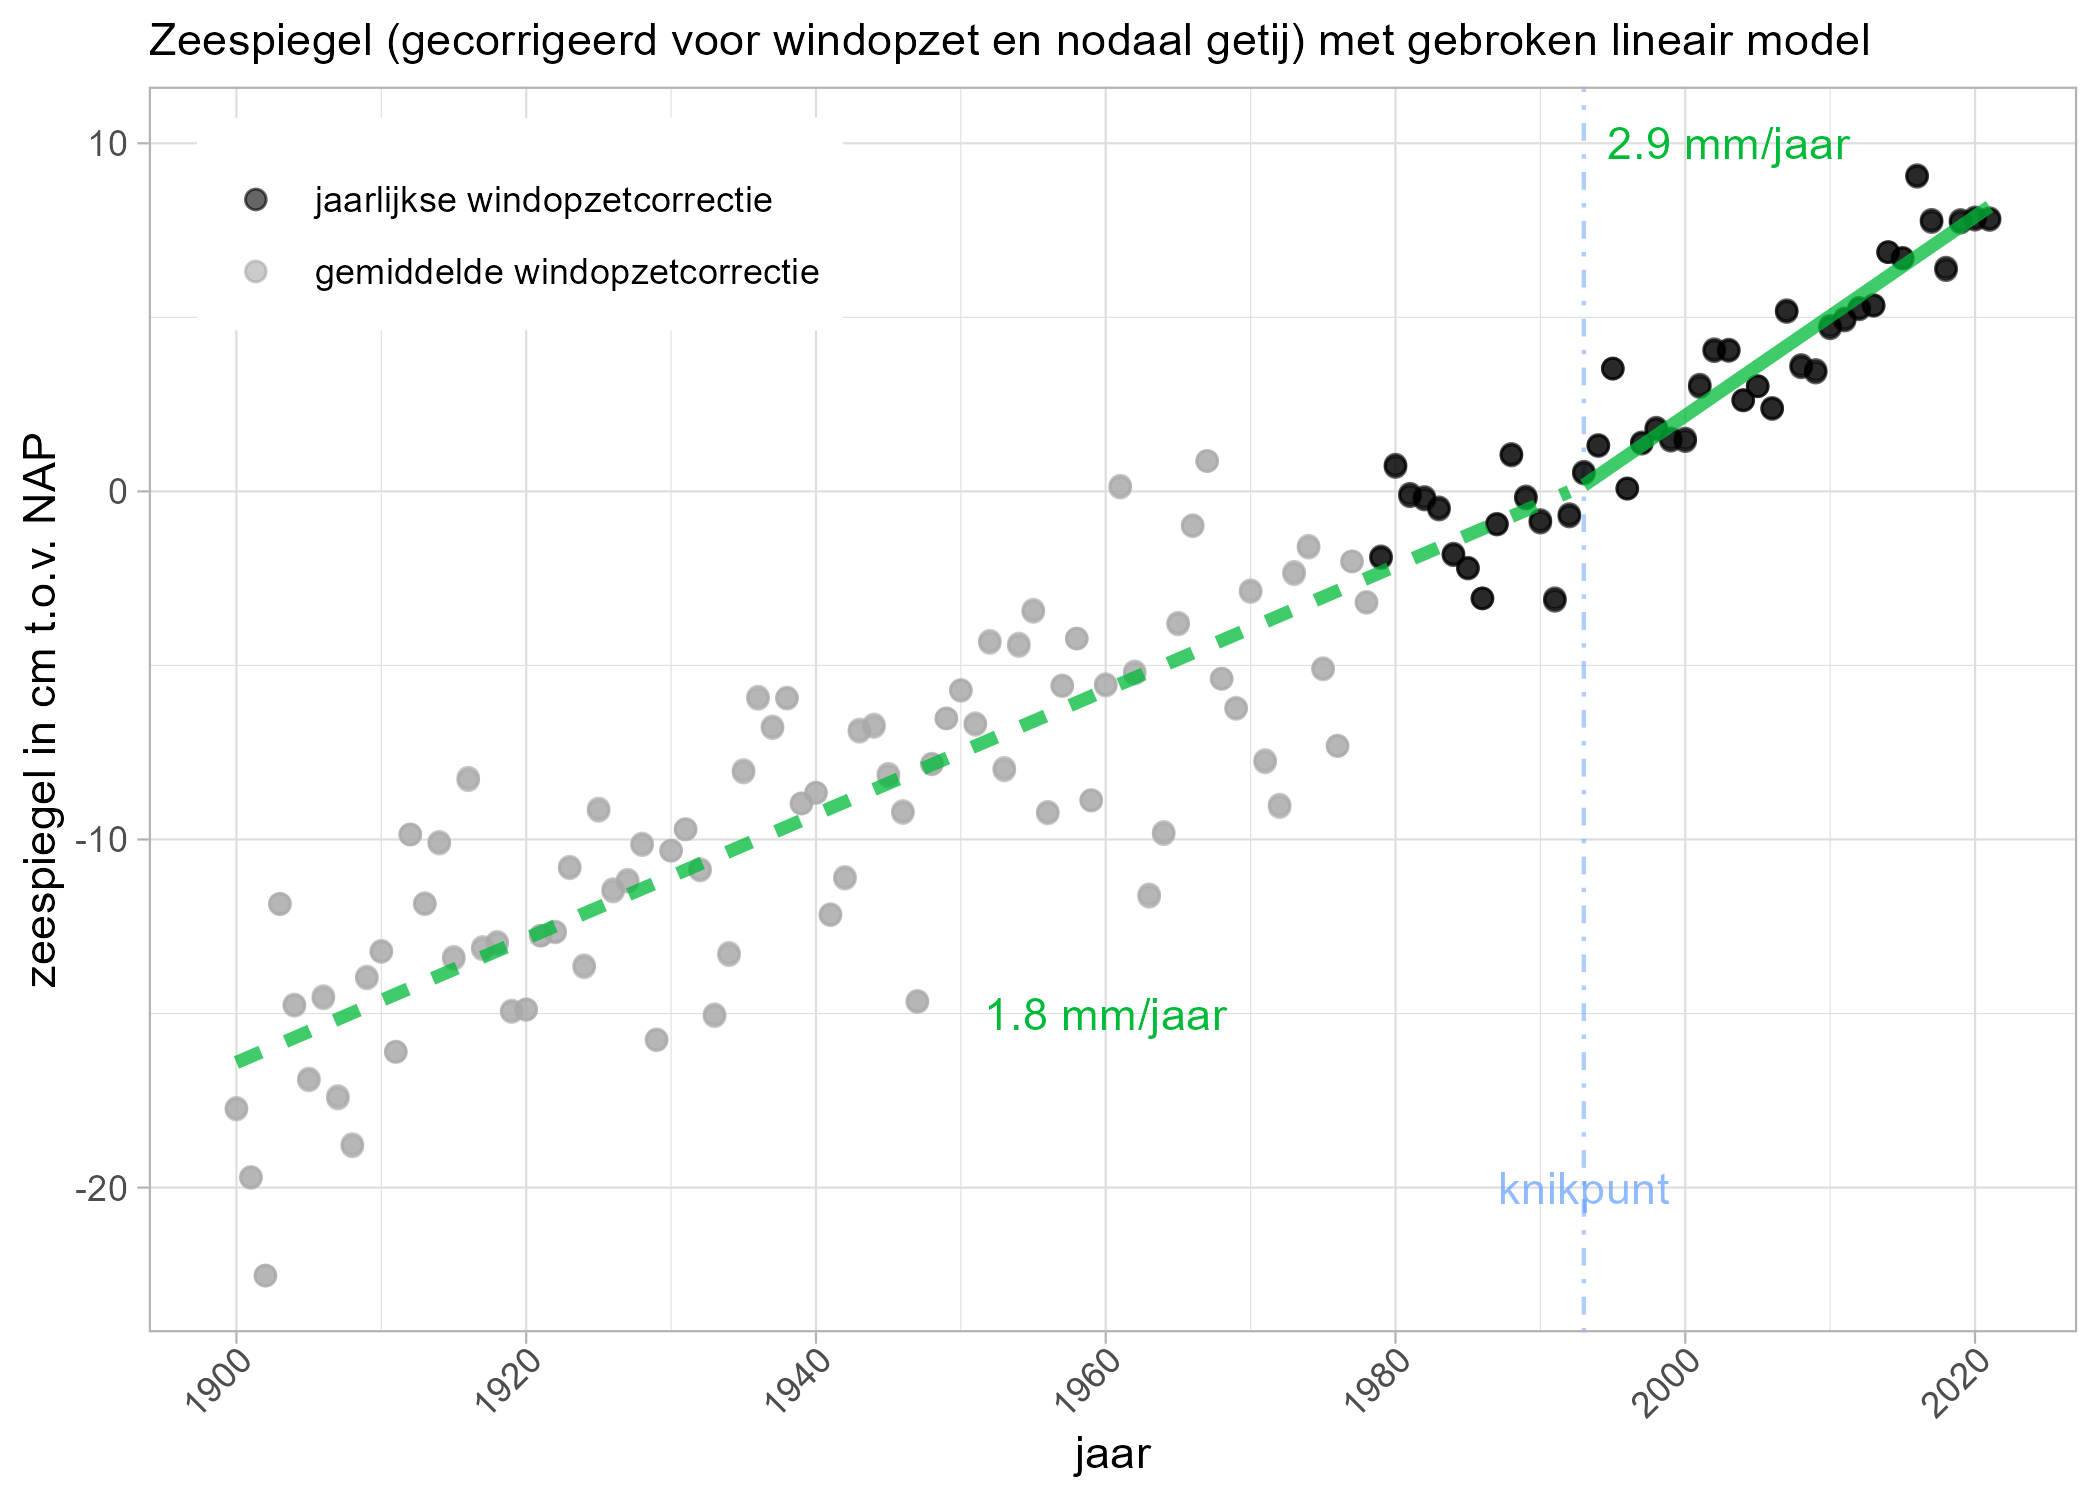
\includegraphics[width=0.7\linewidth]{figures/samenvatting_v2} 

}

\caption{De verandering van de zeespiegeltrend in de tijd.}\label{fig:unnamed-chunk-2}
\end{figure}

Uit bovenstaande figuur zijn drie belangrijke boodschappen te halen:

\begin{itemize}
\tightlist
\item
  In Nederland is een versnelling van de zeespiegelstijging waarneembaar. De stijging is in de komende decennia naar verwachting hoger dan de trend in de vorige eeuw.
\item
  De gegevens vanaf 1979 vertonen een kleinere onzekerheid dan daarvoor. Dit komt door een meer nauwkeurige correctie voor windopzet. Dat verhoogt de nauwkeurigheid van de beschrijving van de lokale zeespiegelstijging in recente tijdvakken.
\item
  De jaar op jaar variatie van de zeespiegel (ca. ± 10 cm) is veel groter dan de onzekerheid in de langjarige trend (ca. ± 0.4 mm/jaar).
\end{itemize}

In deze zeespiegelmonitor zijn de gegevens van vijf van de zes Nederlandse stations gebruikt. Er is namelijk reden om aan te nemen dat de gegevens van het station Delfzijl nu niet betrouwbaar genoeg zijn, met name veroorzaakt door de snelle bodemdaling. De overige stations vertonen onderling vergelijkbare trends in de stijging sinds 1993, namelijk tussen 2.3 en 3.3 mm per jaar.
}
\deltarestitle
%------------------------------------------------------------------------------

% Text body

$body$

%------------------------------------------------------------------------------
\end{document}
